\Variant{04.10.2026 (2-smena)}
\QQ{1}{$12+122+1332+14862+161061$ ni $11$ ga bölganda hosil böladigan qoldiqni toping.
\Opts{$3$}{$2$}{$7$}{$1$}}
\QQ{2}{$\dfrac{13}{27}$ kasrni çeksiz davriy önli kasr körinişida ifodalang.
\Opts{$0{,}(481)$}{$0{,}(403)$}{$0{,}(476)$}{$0{,}(507)$}}
\QQ{3}{$A$ va $B$ şaharlari orasidagi masofa $70$ km. Birinçi velosipedçi $A$ şahridan $B$ şahri tomon $12$ km/soat tezlik bilan yölga çiqdi. Oradan bir soat ötgaç, ikkinçi velosipedçi ham şu yönalişda $10$ km/soat tezlik bilan harakatlana boşladi. Yana bir soatdan söng uçinçi velosipedçi $A$ şahridan $B$ şahri tomon yölga çiqdi. Uçinçi velosipedçi dastlab ikkinçi velosipedçini, undan ikki soat ötgaç esa birinçi velosipedçini quvib ötdi. Barça velosipedçilar özgarmas tezlik bilan harakatlangan bölsa, uçinçi velosipedçi $B$ şahriga yetib kelgan paytda birinçi va ikkinçi velosipedçilar orasidagi masofani toping.
\Opts{$19$}{$20$}{$21$}{$23$}}
\QQ{4}{Sotuvçi ikkita qadimiy buyumni jami $35$ million sömga sotib, ularni xarid qilişga sarflagan mablağiga nisbatan $40\%$ foyda oldi. Birinçi buyumni xarid narxidan $25\%$, ikkinçi buyumni esa $50\%$ qimmatga sotgan bölsa, ikkinçi buyumning xarid narxini toping.
\Opts{$12\,000\,000$}{$12\,500\,000$}{$15\,000\,000$}{$10\,000\,000$}}
\QQ{5}{Hisoblang: $\sqrt[3]{(-5)^3}-\sqrt[3]{-5^3}+\sqrt{(-5)^2}$.
\Opts{$5$}{$-5$}{$10$}{$-10$}}
\QQ{6}{Hisoblang: $\sqrt[3]{2\sqrt2-4}\cdot\sqrt[3]{2\sqrt2+4}$.
\Opts{$2$}{$-8$}{$8$}{$-2$}}
\QQ{7}{Hisoblang:
\[30\sqrt[3]{\frac1{12}}+3\frac12\sqrt[3]{\frac23}+5\sqrt[3]{144}\]
\Opts{$\dfrac{97\sqrt[3]{12}}6$}{$\dfrac{97\sqrt[3]{18}}6$}{$16\sqrt[3]{12}$}{$16\sqrt[3]{18}$}}
\QQ{8}{Arifmetik progressiyada $a_1+a_3+a_5+\ldots+a_{21}=a_2+a_4+a_6+\ldots+a_{20}$ bölsa, $S_{21}$ ning qiymatini toping.
\Opts{$0$}{$21$}{$-21$}{$221$}}
\QQ{9}{Geometrik progressiyada $b_1+b_2+b_3=224$, $b_4+b_5+b_6=28$ bölsa, $b_7+b_8$ ni toping.
\Opts{$5$}{$12$}{$3$}{$6$}}
\QQ{10}{Ifodani soddalaştiring:
\[\frac{a^2+ab+b^2}{a+b}-\frac{a^2-ab+b^2}{b-a}\]
\Opts{$2a$}{$2b$}{$\dfrac{2a^3}{a^2-b^2}$}{$\dfrac{2b^3}{a^2-b^2}$}}
\QQ{11}{Agar $a=2$ va $b=4$ bölsa, quyidagi ifodaning qiymatini toping:
\[\left(\frac{a^{\frac14}-b^{\frac14}}{a^{\frac12}+a^{\frac14}b^{\frac14}}+\frac{a^{\frac14}+b^{\frac14}}{a^{\frac12}-a^{\frac14}b^{\frac14}}-\frac{2b^{\frac12}}{a^{\frac34}-a^{\frac14}b^{\frac12}}\right)\left(b^{\frac12}-a^{\frac12}\right)\]
\Opts{$2\sqrt2$}{$-2\sqrt[4]2$}{$2\sqrt[4]2$}{$-2\sqrt2$}}
\QQ{12}{Tengsizlikni yeçing: $\arccos x\ge\arcsin x$.
\Opts{$\left[\dfrac{\sqrt2}2;\,1\right]$}{$\left[-\dfrac{\sqrt2}2;\,1\right]$}{$\left[0;\,\dfrac{\sqrt2}2\right]$}{$\left[-1;\,\dfrac{\sqrt2}2\right]$}}
\QQ{13}{Tengsizlikni yeçing:
\[2\sin\frac x2\cos\frac x2+\sin^2\frac x2\ge\cos^2\frac x2\]
\Opts{$\left[\dfrac\pi4+\pi k;\,\dfrac{3\pi}4+\pi k\right]$}{$\left[-\dfrac\pi4+2\pi k;\,\dfrac{3\pi}4+2\pi k\right]$}{$\left[\dfrac\pi4+2\pi k;\,\dfrac{5\pi}4+2\pi k\right]$}{$\left[\dfrac{3\pi}4+2\pi k;\,\dfrac{7\pi}4+2\pi k\right]$}}
\QQ{14}{Tenglama neçta haqiqiy yeçimga ega?
\[7^{2x+3}=5^{2x^2+3x-5}\]
\Opts{$3$ ta}{$1$ ta}{$2$ ta}{yeçimga ega emas}}
\QQ{15}{Tengsizlikni qanoatlantiruvçi butun sonlar sonini toping:
\[1+\log_{0{,}25}\bigl(\log_3(4-x)\bigr)>0\]
\Opts{$72$}{$75$}{çeksiz köp}{$79$}}
\QQ{16}{Tenglama neçta haqiqiy ildizga ega?
\[\left(\frac x{x-1}\right)^2+\left(\frac x{x+1}\right)^2=90\]
\Opts{$1$ ta}{$2$ ta}{$3$ ta}{$4$ ta}}
\QQ{17}{Tenglamaning haqiqiy ildizlari yiğindisini toping:
\[x^2+16=\frac{10x^2-20x}{x-2}\]
\Opts{$8$}{$10$}{$2$}{$16$}}
\QQ{18}{Tengsizlikni yeçing:
\[\frac{|x-1|}{3-x}\ge\frac{|1-x|}{3-2x}\]
\Opts{$(-\infty;\,0]\cup(1{,}5;\,3)$}{$[0;\,1{,}5)\cup(3;\,\infty)$}{$(-\infty;\,0]\cup\{1\}\cup(1{,}5;\,3)$}{$(-\infty;\,1]\cup(1{,}5;\,3)$}}
\QQ{19}{Tengsizlikning butun yeçimlari neçta?
\[\sqrt{x+5}+\sqrt{2-x}>\sqrt{3x+1}\]
\Opts{$2$}{$3$}{$1$}{yeçimga ega emas}}
\QQ{20}{Funksiyaning kamayiş oraliğini toping:
\[f(x)=\frac{(x-1)\sqrt{x^2-6x+5}}{x-1}\]
\Opts{$(-\infty;\,1)$}{$(5;\,\infty)$}{$(-\infty;\,3)$}{$(-\infty;\,5)$}}
\QQ{21}{Aniq integralni hisoblang:
\[\int\limits_{-4}^4\frac{dx}{\sqrt{\left(x^2+9\right)^3}}\]
\Opts{$\dfrac8{45}$}{$0$}{$\dfrac4{45}$}{$\dfrac2{15}$}}
\QQ{22}{Koordinata tekisligida $A\left(0;\,\dfrac52\right)$ nuqta va $y=\dfrac{x^4}8$ funksiya berilgan. $A$ nuqtadan uşbu funksiya grafigigaça bölgan eng qisqa masofani toping.
\Opts{$\dfrac{\sqrt{17}}2$}{$\sqrt{\dfrac{17}2}$}{$\sqrt{\dfrac{13}2}$}{$\dfrac{\sqrt{17}}4$}}
\QQ{23}{Aylanaga ötkazilgan vatar aylana markazidan $90^\circ$ li yoyni tortib turibdi. Agar aylana radiusi $8$ ga teng bölsa, vatar uzunligini toping.
\qfig{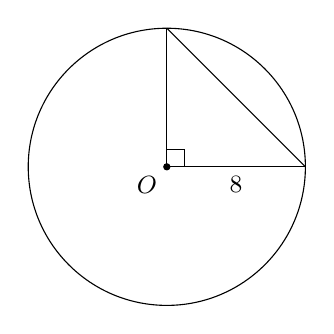
\begin{tikzpicture}[scale=0.22,font=\small]
\draw (0,0) circle (8); \draw (0,0)--(8,0); \draw (0,0)--(0,8); \draw (8,0)--(0,8); \fill (0,0) circle (6pt);
\draw (0,1)--(1,1)--(1,0); \node[below] at (4,0) {$8$}; \node[below left] at (0,0) {$O$};
\end{tikzpicture}}
\Opts{$8\sqrt2$}{$4\sqrt2$}{$8$}{$4$}}
\QQ{24}{$f(x)=x^5+x^2-9x+8$ funksiyani $Ox$ öqi böylab $3$ birlik öngga, $Oy$ öqi böylab $2$ birlik yuqoriga siljitiş natijasida hosil bölgan funksiya $g(x)$ bölsa, $g(2)$ ning qiymatini toping.
\Opts{$17$}{$19$}{$15$}{$26$}}
\QQ{25}{$ABC$ uçburçakning $AB$ tomonida $D$ nuqta olingan. $BE$ kesma $\angle ABC$ ning bissektrisasi bölib, $E$ nuqta $AC$ tomonida yotadi. Agar $\angle BAC=45^\circ$, $\angle ACD=15^\circ$ va $\angle BCD=60^\circ$ bölsa, $\angle DEB$ ning kattaligini toping.
\qfig{\begin{tikzpicture}[scale=0.6,font=\small]
\coordinate (A) at (0,0); \coordinate (C) at (8,0); \coordinate (B) at (6.309,6.309); \coordinate (D) at (1.691,1.691); \coordinate (E) at (4.619,0);
\draw (A)--(B)--(C)--cycle; \draw (B)--(E); \draw (D)--(C); \draw (D)--(E);
\draw (0.8,0) arc (0:45:0.8); \node at (1.2,0.45) {\tiny$45^\circ$};
\draw (6.7,0) arc (180:165:1.3); \node at (6.3,0.2) {\tiny$15^\circ$};
\draw ($(C)+(165:0.6)$) arc (165:105:0.6); \node at (7.35,0.95) {\tiny$60^\circ$};
\node[below left] at (A) {$A$}; \node[above] at (B) {$B$}; \node[below right] at (C) {$C$}; \node[above left] at (D) {$D$}; \node[below] at (E) {$E$};
\end{tikzpicture}}
\Opts{$72^\circ$}{$65^\circ$}{$60^\circ$}{$75^\circ$}}
\QQ{26}{$ABC$ uçburçakning $B$ uçidan $AC$ tomoniga $BH$ balandlik va $BM$ mediana ötkazilgan. Agar $AC=56$, $MH=14$ va $\angle MBC=40^\circ$ bölsa, $\angle AMB$ ning kattaligini toping.
\Opts{$100^\circ$}{$120^\circ$}{$130^\circ$}{$110^\circ$}}
\QQ{27}{$ABCD$ parallelogrammning $AB$ tomonidan $E$ va $F$ nuqtalar, $CD$ tomonidan esa $M$ va $N$ nuqtalar olingan. Bunda $2AE=2BF=EF$ va $CM=MN=ND$. $FN$ va $EM$ kesmalar $O$ nuqtada kesişadi. Böyalgan $EFO$ va $MNO$ uçburçaklar yuzalari yiğindisining $ABCD$ parallelogramm yuziga nisbatini toping.
\qfig{\begin{tikzpicture}[scale=0.85,font=\small]
\coordinate (A) at (0,0); \coordinate (B) at (0.5,3); \coordinate (C) at (4.5,3); \coordinate (D) at (4,0);
\coordinate (E) at (0.125,0.75); \coordinate (F) at (0.375,2.25); \coordinate (M) at (4.333,2); \coordinate (N) at (4.167,1);
\coordinate (O) at (intersection of F--N and E--M);
\fill[qfill] (E)--(F)--(O)--cycle; \fill[qfill] (M)--(N)--(O)--cycle;
\draw (A)--(B)--(C)--(D)--cycle; \draw (F)--(N); \draw (E)--(M);
\foreach \p in {A,B,C,D,E,F,M,N} \fill (\p) circle (1.2pt);
\node[below left] at (A) {$A$}; \node[above left] at (B) {$B$}; \node[above right] at (C) {$C$}; \node[below right] at (D) {$D$};
\node[left] at (E) {$E$}; \node[left] at (F) {$F$}; \node[right] at (M) {$M$}; \node[right] at (N) {$N$}; \node[above] at (O) {$O$};
\end{tikzpicture}}
\Opts{$\dfrac7{60}$}{$\dfrac{13}{60}$}{$\dfrac14$}{$\dfrac15$}}
\QQ{28}{Muntazam uçburçak tomoni $9$ ga teng. Uçburçak içiga uçta teng muntazam oltiburçak çizilgan. Böyalgan soha yuzini toping.
\qfig{\begin{tikzpicture}[scale=0.42,font=\small]
\foreach \cx/\cy in {-1.5/1.732,1.5/1.732,0/4.330} {\fill[qfill] ($(\cx,\cy)+(90:1.732)$)--($(\cx,\cy)+(150:1.732)$)--($(\cx,\cy)+(210:1.732)$)--($(\cx,\cy)+(270:1.732)$)--($(\cx,\cy)+(330:1.732)$)--($(\cx,\cy)+(30:1.732)$)--cycle;
\draw ($(\cx,\cy)+(90:1.732)$)--($(\cx,\cy)+(150:1.732)$)--($(\cx,\cy)+(210:1.732)$)--($(\cx,\cy)+(270:1.732)$)--($(\cx,\cy)+(330:1.732)$)--($(\cx,\cy)+(30:1.732)$)--cycle;}
\draw (-4.5,0)--(4.5,0)--(0,7.794)--cycle; \node[left] at (-2.4,3.9) {$9$};
\end{tikzpicture}}
\Opts{$9$}{$3$}{$\dfrac{9\sqrt3}2$}{$\dfrac{27\sqrt3}2$}}
\QQ{29}{Koordinata tekisligida uçlari $A(0;\,0)$, $B(1;\,2)$, $C(3;\,3)$ va $D(4;\,0)$ nuqtalarda joylaşgan qavariq $ABCD$ törtburçak berilgan. $CD$ tomonida şunday $E$ nuqta olinganki, $AE$ kesma törtburçak yuzini teng ikkiga böladi. $E$ nuqtaning koordinatalarini toping.
\Opts{$\left(\dfrac{15}8;\,\dfrac{27}8\right)$}{$\left(\dfrac72;\,\dfrac32\right)$}{$\left(\dfrac{27}8;\,\dfrac{15}8\right)$}{$\left(\dfrac{16}{13};\,\dfrac{24}{13}\right)$}}
\QQ{30}{Muntazam törtburçakli piramidaning yon sirtining yuzi $144\sqrt2$ ga teng. Piramidaning apofemasi asos tekisligi bilan $45^\circ$ burçak taşkil qiladi. Piramidaning hajmini toping.
\Opts{$144$}{$288$}{$432$}{$864$}}
\QQ{31}{Rasmdagi maʼlumotlar asosida $(A\cup C)\setminus B'$ töplamning elementlari sonini toping. ($B'$ — $B$ töplamning töldiruvçisi.)
\qfig{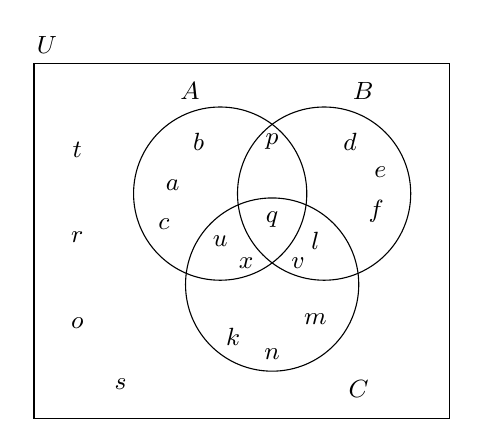
\begin{tikzpicture}[scale=1.1,font=\small]
\draw (-2.9,-2.1) rectangle (1.9,2.0); \node[above] at (-2.75,2.0) {$U$};
\draw (-0.75,0.5) circle (1); \draw (0.45,0.5) circle (1); \draw (-0.15,-0.55) circle (1);
\node at (-1.1,1.68) {$A$}; \node at (0.9,1.68) {$B$}; \node at (0.85,-1.75) {$C$};
\foreach \t/\x/\y in {a/-1.3/0.6,b/-1.0/1.1,c/-1.4/0.15,p/-0.15/1.1,d/0.75/1.1,e/1.1/0.75,f/1.05/0.3,q/-0.15/0.2,u/-0.75/-0.05,x/-0.45/-0.3,l/0.35/-0.05,v/0.15/-0.3,k/-0.6/-1.15,n/-0.15/-1.35,m/0.35/-0.95,t/-2.4/1,r/-2.4/0,o/-2.4/-1,s/-1.9/-1.7} \node at (\x,\y) {$\t$};
\end{tikzpicture}}
\Opts{$4$}{$3$}{$5$}{$6$}}
\QQ{32}{$a$, $b$ va $c$ raqamlari özaro turliça bölsa, $\overline{abca}$ körinişidagi neçta tört xonali son mavjud?
\Opts{$720$}{$729$}{$648$}{$680$}}
\QQ{33}{\Moslash{Kub va öq kesimi kvadrat bölgan silindr berilgan. ($\pi\approx3$ deb olinsin.)
\par\centering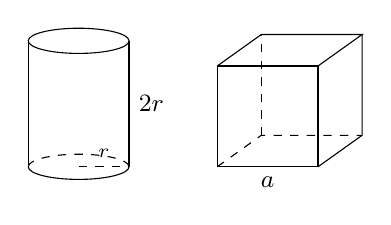
\begin{tikzpicture}[scale=0.8,font=\small]
\draw (0,2) ellipse (0.8 and 0.2); \draw (-0.8,0)--(-0.8,2); \draw (0.8,0)--(0.8,2); \draw (-0.8,0) arc (180:360:0.8 and 0.2); \draw[dashed] (0.8,0) arc (0:180:0.8 and 0.2);
\draw[dashed] (0,0)--(0.8,0); \node[above] at (0.4,0) {\scriptsize$r$}; \node[right] at (0.8,1) {$2r$};
\begin{scope}[xshift=2.2cm]
\draw (0,0) rectangle (1.6,1.6); \draw (0,1.6)--(0.7,2.1)--(2.3,2.1)--(1.6,1.6); \draw (2.3,2.1)--(2.3,0.5)--(1.6,0);
\draw[dashed] (0,0)--(0.7,0.5)--(2.3,0.5); \draw[dashed] (0.7,0.5)--(0.7,2.1); \node[below] at (0.8,0) {$a$};
\end{scope}
\end{tikzpicture}}{A) $\dfrac34$\par B) $\dfrac13$\par C) $\dfrac16$\par D) $\dfrac23$\par E) $1$\par F) $\dfrac12$}{Silindr va kubning hajmlari teng bölsa, silindr töla sirtining kub töla sirtiga nisbatining kubini toping.}{Kub va silindrning yon sirtlari teng bölsa, kubning bitta yoği yuzini silindr bitta asosi yuziga nisbatini toping.}{Kub qirrasi silindr radiusiga teng bölsa, kub hajmini silindr hajmiga nisbatini toping.}}
\QQ{36}{Parametrli tenglama berilgan:
\[\left(x^2+3x+k\right)\left(x^2+9x+k\right)+8x^2=0\]
\AB{Tenglama $2$ ta haqiqiy ildizga ega böladigan $k$ ning barça butun qiymatlari yiğindisini hisoblang.}{Tenglama $4$ ta haqiqiy ildizga ega böladigan $k$ ning eng katta butun qiymatini toping.}}
\QQ{37}{Tenglamani yeçing:
\[8\cos\frac{3x}4\cos\frac x4-6\cos x+1=0\]
\AB{Tenglamaning eng kiçik musbat ildizini toping.}{Tenglama $(-2\pi;\,2\pi)$ oraliqda neçta yeçimga ega?}}
\QQ{38}{$f(x)$ funksiya uçun $3f(-x)+f(x)+f\left(\dfrac1x\right)=x$ tenglik örinli bölsa,
\AB{$f(1)$ ning qiymatini toping.}{Agar $f(x)=1$ tenglamaning ildizlari $x_1$ va $x_2$ bölsa, $\dfrac1{x_1^3}+\dfrac1{x_2^3}$ ning qiymatini toping.}}
\QQ{39}{Agar $f(3x+1)=x^3-3x^2+12x-1$ va $g(1-2x)=2x-x^2$ bölsa,
\AB{$\dfrac{f'(4)}{g'(-3)}$ ni toping.}{$f'\bigl(g(-7)\bigr)$ ni toping.}}
\QQ{40}{Rasmda $y=ax^2+bx+c$ parabola va $y=3x-4$ töğri çiziqning grafiklari tasvirlangan. Parabola $Ox$ öqini $(-2;\,0)$ va $(4;\,0)$ nuqtalarda, $Oy$ öqini esa $(0;\,8)$ nuqtada kesib ötadi. Parabola bilan töğri çiziqning abssissasi musbat bölgan kesişiş nuqtasi $A(m;\,n)$ deb belgilangan.
\qfig{\begin{tikzpicture}[xscale=0.55,yscale=0.16,font=\small]
\fill[qfill] plot[domain=-4:3,samples=60] (\x,{-\x*\x+2*\x+8})--(-4,-16)--cycle;
\draw[-{Stealth[length=4pt]}] (-5,0)--(5.2,0) node[right] {$x$}; \draw[-{Stealth[length=4pt]}] (0,-20)--(0,12.5) node[left] {$y$};
\draw[thick,domain=-4.25:4.3,samples=80] plot (\x,{-\x*\x+2*\x+8}); \draw[thick] (-4.4,-17.2)--(3.9,7.7);
\fill (3,5) circle (4.5pt); \fill (0,8) circle (4.5pt); \node[right] at (3.1,5.5) {\scriptsize$A(m;\,n)$}; \node[above left] at (0,8) {\scriptsize$8$};
\node[below left] at (-2,0) {\scriptsize$-2$}; \node[below right] at (4,0) {\scriptsize$4$};
\node[left] at (-1.3,10.5) {\scriptsize$y=ax^2+bx+c$}; \node[right] at (1.3,-5) {\scriptsize$y=3x-4$};
\end{tikzpicture}}
\AB{$\dfrac{a+b+c}{m+n}$ ni toping.}{Böyalgan soha yuzini toping.}}
\QQ{41}{Radiusi $4\sqrt3$ ga teng bölgan aylanaga $ABC$ uçburçak içki çizilgan. Uçburçakning $AB$ tomoni $8$ ga, $\angle BAC=60^\circ$. $AB$ va $BC$ tomonlarning örtalari mos ravişda $D$ va $E$ nuqtalar bilan belgilangan. $DE$ töğri çiziq aylanani $G$ va $F$ nuqtalarda kesib ötadi.
\qfig{\begin{tikzpicture}[scale=0.3,font=\small]
\coordinate (A) at (-4,-5.657); \coordinate (B) at (4,-5.657); \coordinate (C) at (2.899,6.292); \coordinate (D) at (0,-5.657); \coordinate (E) at (3.449,0.318); \coordinate (F) at (5.611,4.064); \coordinate (G) at (-0.713,-6.891);
\draw (0,0) circle (6.928); \draw (A)--(B)--(C)--cycle; \draw (G)--(F);
\foreach \p in {A,B,C,D,E,F,G} \fill (\p) circle (5pt);
\draw ($(A)+(0:1)$) arc (0:60:1); \node at ($(A)+(30:1.7)$) {\tiny$60^\circ$};
\node[left] at (A) {$A$}; \node[right] at (B) {$B$}; \node[above] at (C) {$C$}; \node[above] at (D) {$D$}; \node[left] at (E) {$E$}; \node[right] at (F) {$F$}; \node[below] at (G) {$G$};
\end{tikzpicture}}
\AB{$DE$ kesma uzunligini toping.}{$GF$ kesma uzunligini toping.}}
\QQ{42}{Rasmda $ABCD$ kvadrat tasvirlangan. $ACD$ uçburçak içidan $E$ nuqta şunday joylaşganki, bunda $AE=\sqrt2$, $DE=3$ va $EC=2\sqrt5$ tengliklar örinli.
\qfig{\begin{tikzpicture}[scale=0.85,font=\small]
\coordinate (A) at (0,0); \coordinate (B) at (0,4.123); \coordinate (C) at (4.123,4.123); \coordinate (D) at (4.123,0); \coordinate (E) at (1.213,0.728);
\fill[qfill] (A)--(C)--(E)--cycle;
\draw (A)--(B)--(C)--(D)--cycle; \draw (A)--(C); \draw (A)--(E)--(C); \draw (E)--(D);
\node[below left] at (A) {$A$}; \node[above left] at (B) {$B$}; \node[above right] at (C) {$C$}; \node[below right] at (D) {$D$}; \node[above left] at (E) {$E$};
\node[below] at (0.6,0.38) {\scriptsize$\sqrt2$}; \node[below] at (2.7,0.38) {\scriptsize$3$}; \node[right] at (2.75,2.3) {\scriptsize$2\sqrt5$};
\end{tikzpicture}}
\AB{$ABCD$ kvadrat yuzini toping.}{$ACE$ uçburçakning yuzini toping.}}
\QQ{43}{$ABC$ uçburçak markazi $O_2$ va radiusi $R$ bölgan aylanaga içki çizilgan. Markazi $O_1$ bölgan kiçik aylana $AB$ va $BC$ tomonlarga urinadi. $O_1$ nuqta $AC$ kesmada yotadi. Kiçik aylana $AC$ kesmani $K$ va $L$ nuqtalarda kesib ötadi. Bunda $AK=2$, $KL=16$ va $LC=9$.
\qfig{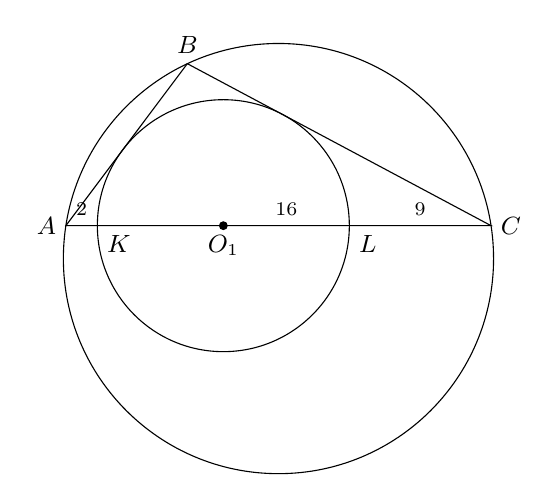
\begin{tikzpicture}[scale=0.2,font=\small]
\coordinate (A) at (0,0); \coordinate (C) at (27,0); \coordinate (B) at (7.714,10.286); \coordinate (K) at (2,0); \coordinate (L) at (18,0); \coordinate (O) at (10,0);
\draw (13.5,-2.089) circle (13.659); \draw (O) circle (8); \draw (A)--(B)--(C)--cycle; \fill (O) circle (8pt);
\node[left] at (A) {$A$}; \node[above] at (B) {$B$}; \node[right] at (C) {$C$}; \node[below right] at (K) {$K$}; \node[below right] at (L) {$L$}; \node[below] at (O) {$O_1$};
\node[above] at (1,0) {\scriptsize$2$}; \node[above] at (14,0) {\scriptsize$16$}; \node[above] at (22.5,0) {\scriptsize$9$};
\end{tikzpicture}}
\AB{$\dfrac{AB}{BC}$ ni toping.}{Uçburçakka taşqi çizilgan aylananing $R$ radiusini toping.}}
\QQ{44}{Şar içiga muntazam uçburçakli kesik piramida çizilgan. Kesik piramidaning asoslari yuzlari $9\sqrt3$ va $81\sqrt3$ ga teng. Uning yon qirrasi bilan asos tekisligi orasidagi burçak $60^\circ$ ni taşkil etadi.
\AB{Kesik piramidaning hajmini toping.}{Şarning radiusini toping.}}
\QQ{45}{Töğri doiraviy kesik konusning kiçik va katta asoslari radiuslari mos ravişda $1$ va $2$ ga teng. Uning yasovçisi katta asos tekisligi bilan $60^\circ$ burçak hosil qiladi. Katta asos aylanasidagi $A$ nuqtada çumoli turibdi. Kiçik asos aylanasidagi $C$ nuqta $A$ nuqtadan ötuvçi öq kesimining qarama-qarşi yasovçisida joylaşgan. ($\pi\approx3$ deb olinsin.)
\qfig{\begin{tikzpicture}[scale=0.9,font=\small]
\draw (-2,0) arc (180:360:2 and 0.35); \draw[dashed] (2,0) arc (0:180:2 and 0.35); \draw (0,1.732) ellipse (1 and 0.18);
\draw (-2,0)--(-1,1.732); \draw (2,0)--(1,1.732); \draw[dashed] (0,0)--(2,0); \draw[dashed] (0,1.732)--(1,1.732);
\draw ($(2,0)+(180:0.35)$) arc (180:120:0.35); \node at (1.45,0.3) {\tiny$60^\circ$};
\fill (-2,0) circle (1.5pt); \fill (1,1.732) circle (1.5pt);
\node[left] at (-2,0) {$A$}; \node[right] at (1,1.8) {$C$}; \node[above] at (0.5,1.732) {\scriptsize$1$}; \node[below] at (1,0) {\scriptsize$2$};
\end{tikzpicture}}
\AB{Kesik konusning yon sirt yuzini toping.}{Çumoli kesik konusning yon sirti böylab $A$ nuqtadan $C$ nuqtaga borişi uçun bosib ötişi kerak bölgan eng qisqa yöl uzunligini toping.}}
\Javoblar{A A C C A D B A C C B D C C D D A C A A A A A B D D B D C B A C A E C}{\OK{36}{$57$}{$6$}\OK{37}{$\dfrac{4\pi}3$}{$2$}\OK{38}{$-1$}{$-9$}\OK{39}{$3$}{$19$}\OK{40}{$\dfrac98$}{$\dfrac{343}6$}\OK{41}{$2+2\sqrt6$}{$4\sqrt{10}$}\OK{42}{$17$}{$1$}\OK{43}{$\dfrac{10}{17}$}{$\dfrac{765}{56}$}\OK{44}{$468\sqrt3$}{$4\sqrt7$}\OK{45}{$18$}{$2\sqrt3+1$}}
